\begin{frame}{Ứng dụng}
  \begin{figure}[H] % places figure environment here   
    \centering % Centers Graphic
    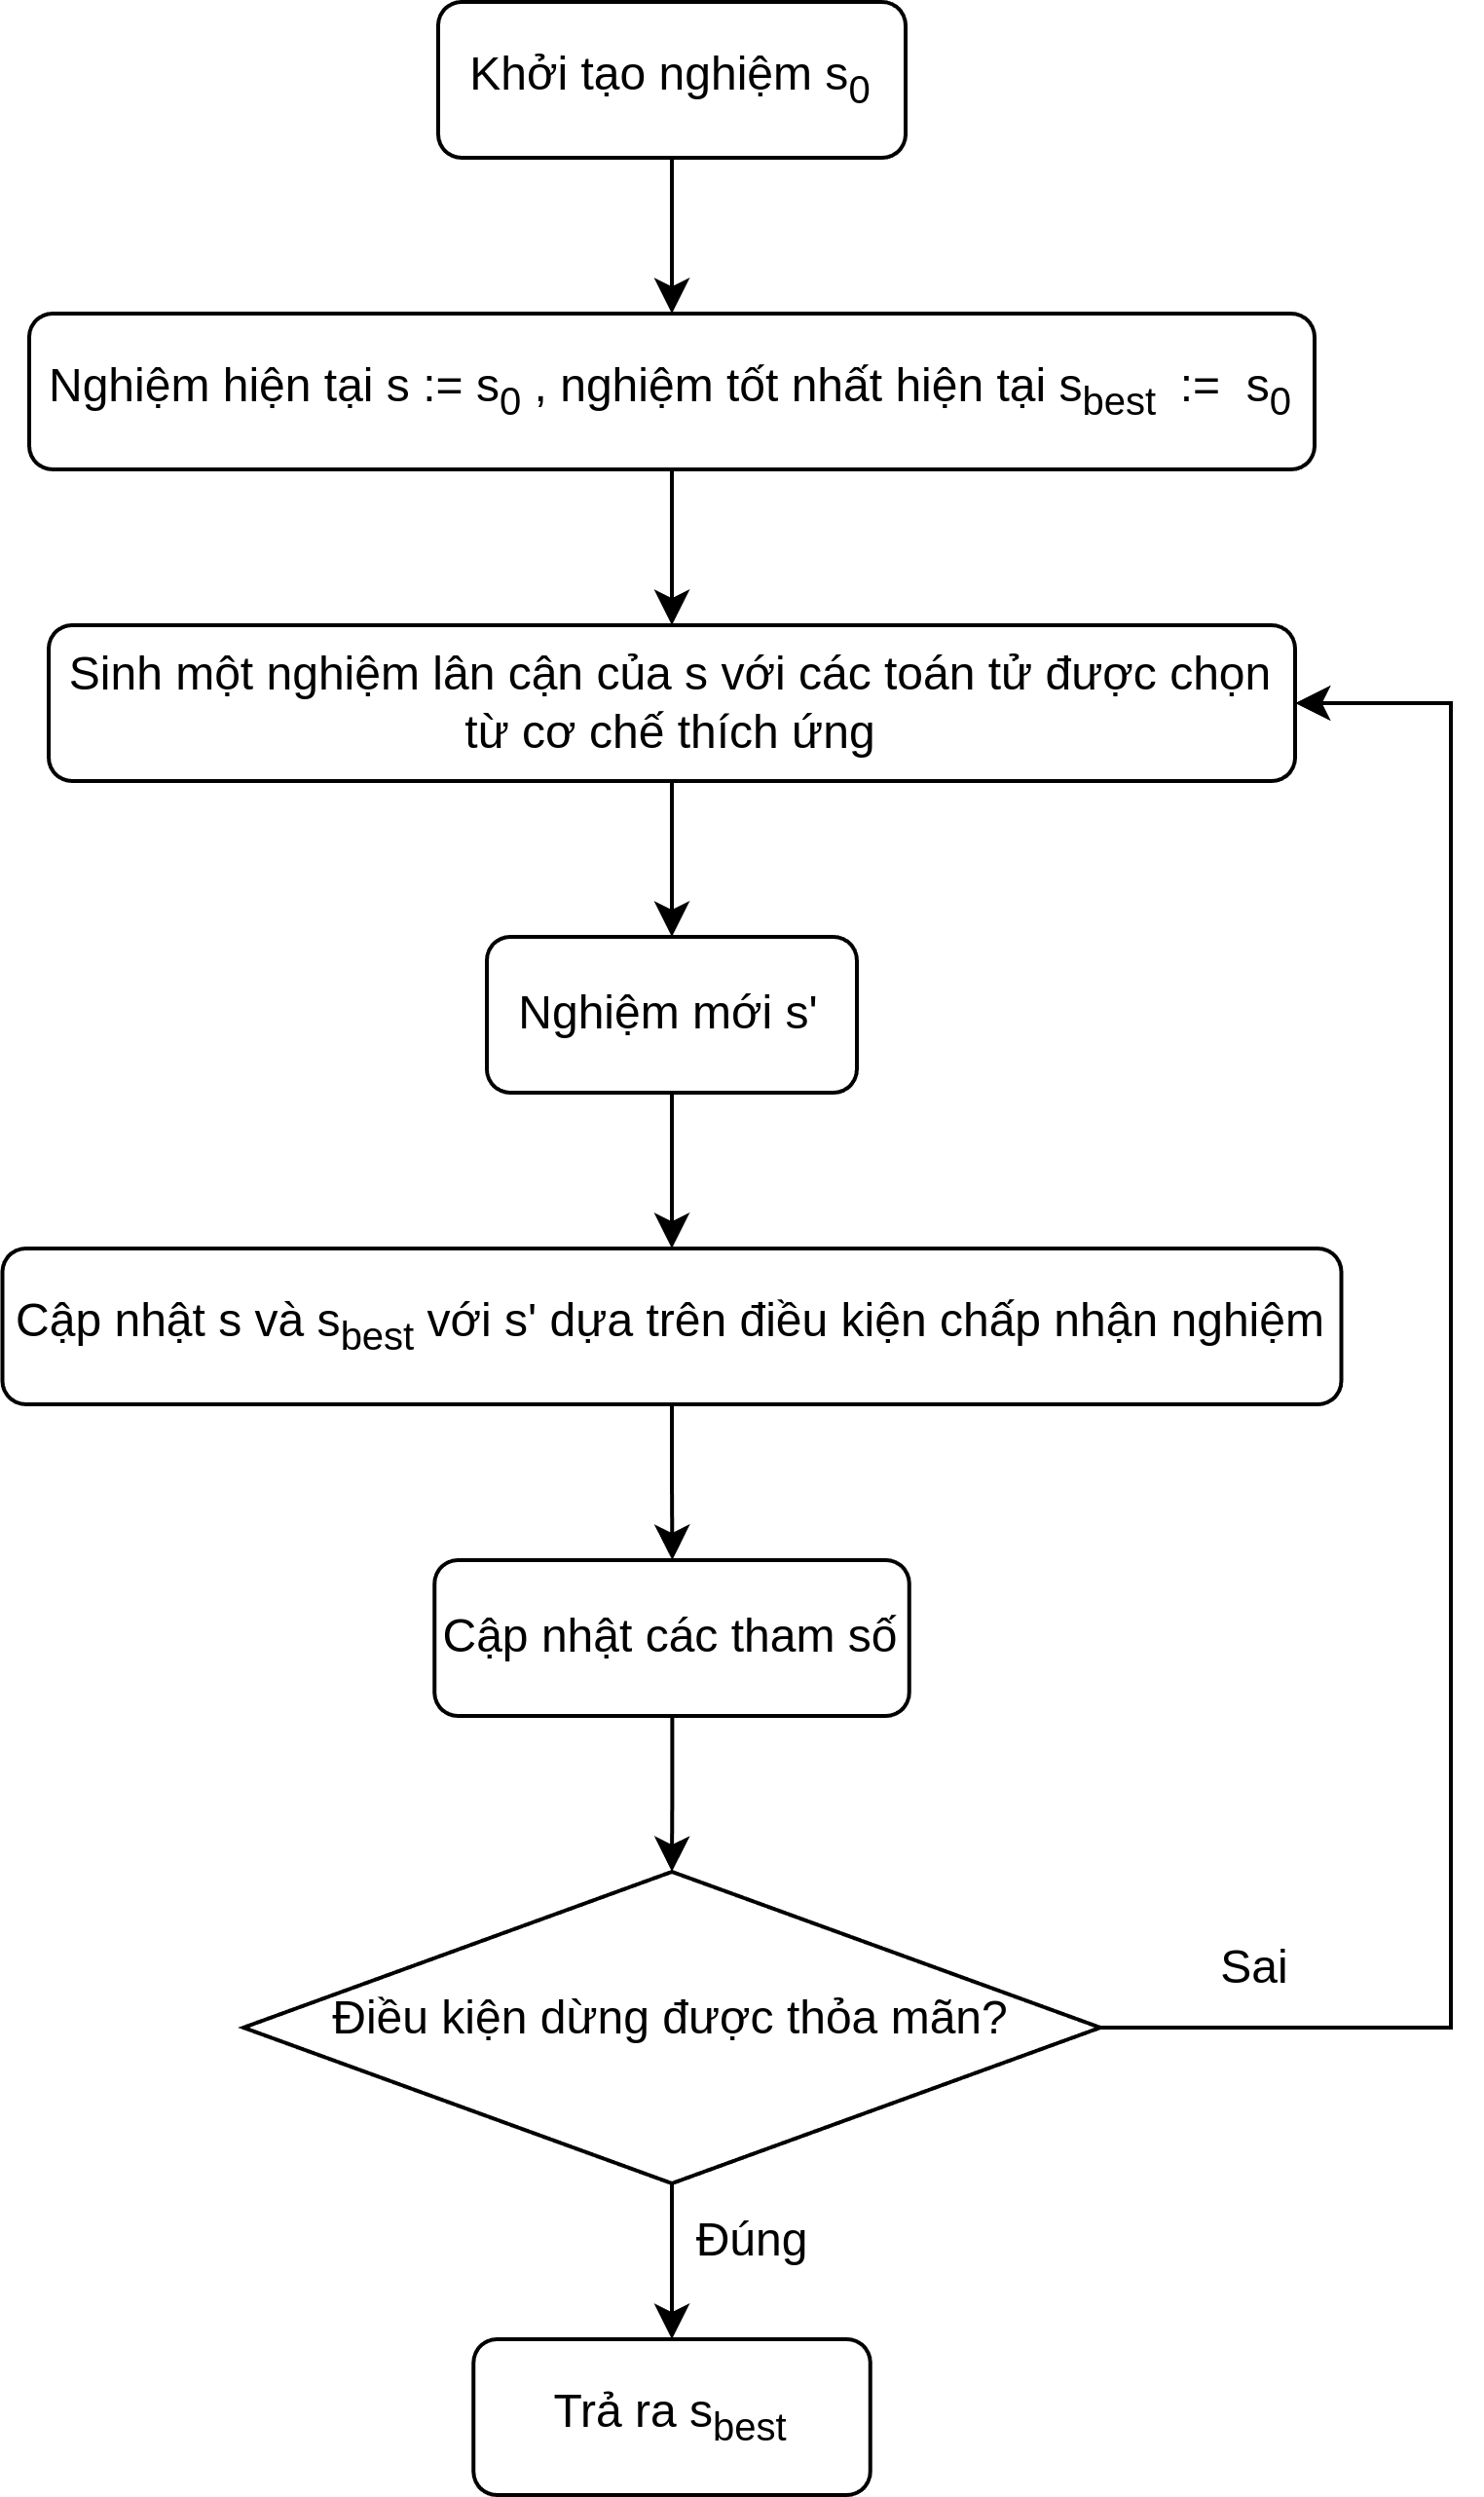
\includegraphics[width=0.3\textwidth]{figures/ALNS-flowchart.png} 
    \caption{Lược đồ chính của ALNS} 
  \end{figure}
\end{frame}

\begin{frame}{Ứng dụng - Các lớp chính}
  \begin{figure}[H] % places figure environment here   
    \centering % Centers Graphic
    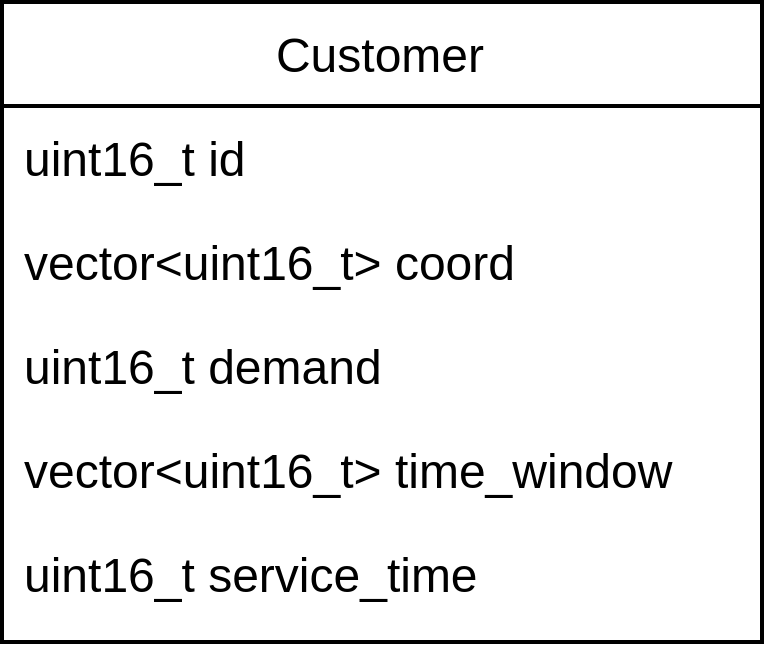
\includegraphics[width=0.35\textwidth]{figures/Customer.png}
    % \includesvg[scale=1]{figures/core-object}
    \caption{Lớp thuộc tính của khách hàng}
    \label{fig:fg_02}
  \end{figure}
\end{frame}

\begin{frame}{Ứng dụng - Các lớp chính}
  \begin{figure}[H] % places figure environment here   
    \centering % Centers Graphic
    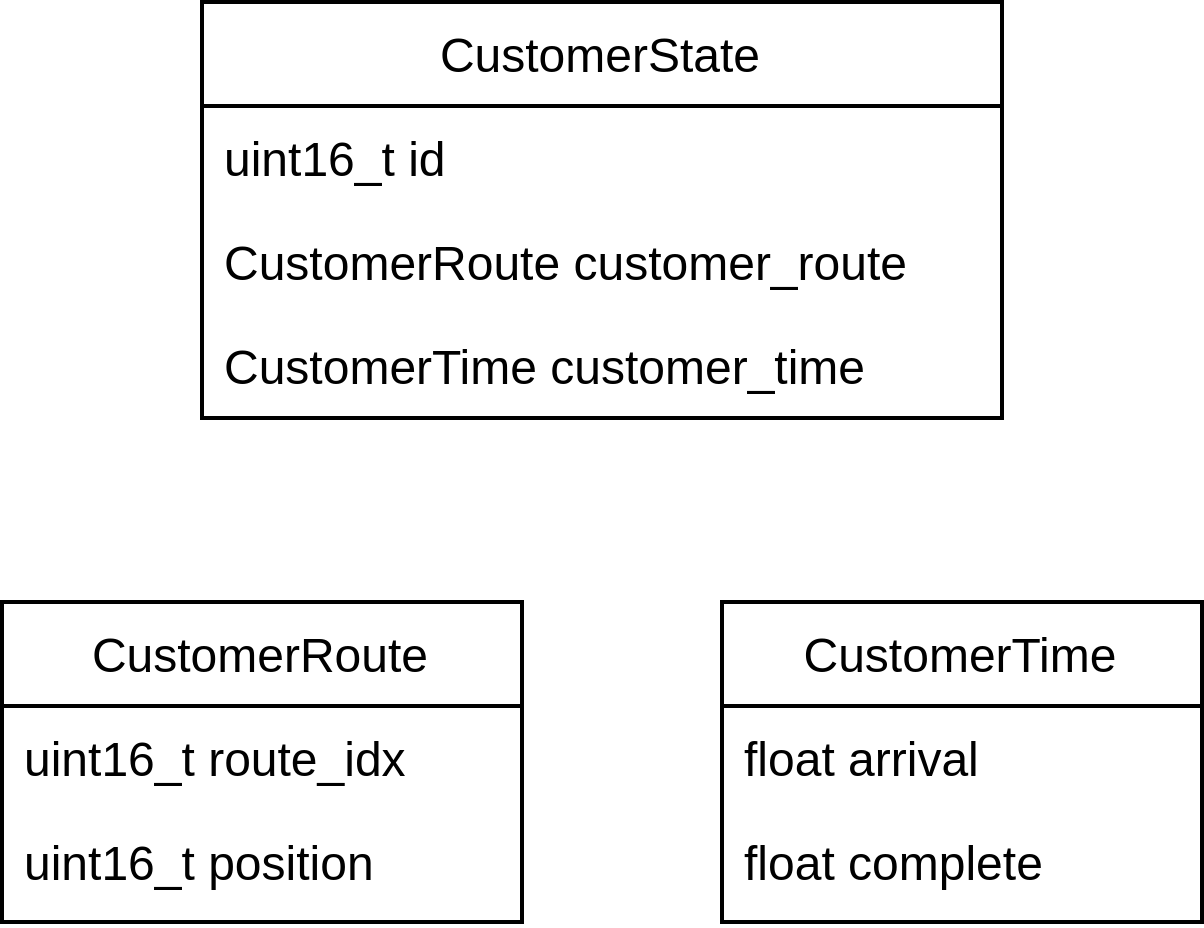
\includegraphics[width=0.6\textwidth]{figures/CustomerState.png}
    % \includesvg[scale=1]{figures/core-object}
    \caption{Lớp trạng thái của khách hàng}
    \label{fig:fg_03}
  \end{figure}
\end{frame}

\begin{frame}{Ứng dụng - Các lớp chính}
  \begin{figure}[H] % places figure environment here   
    \centering % Centers Graphic
    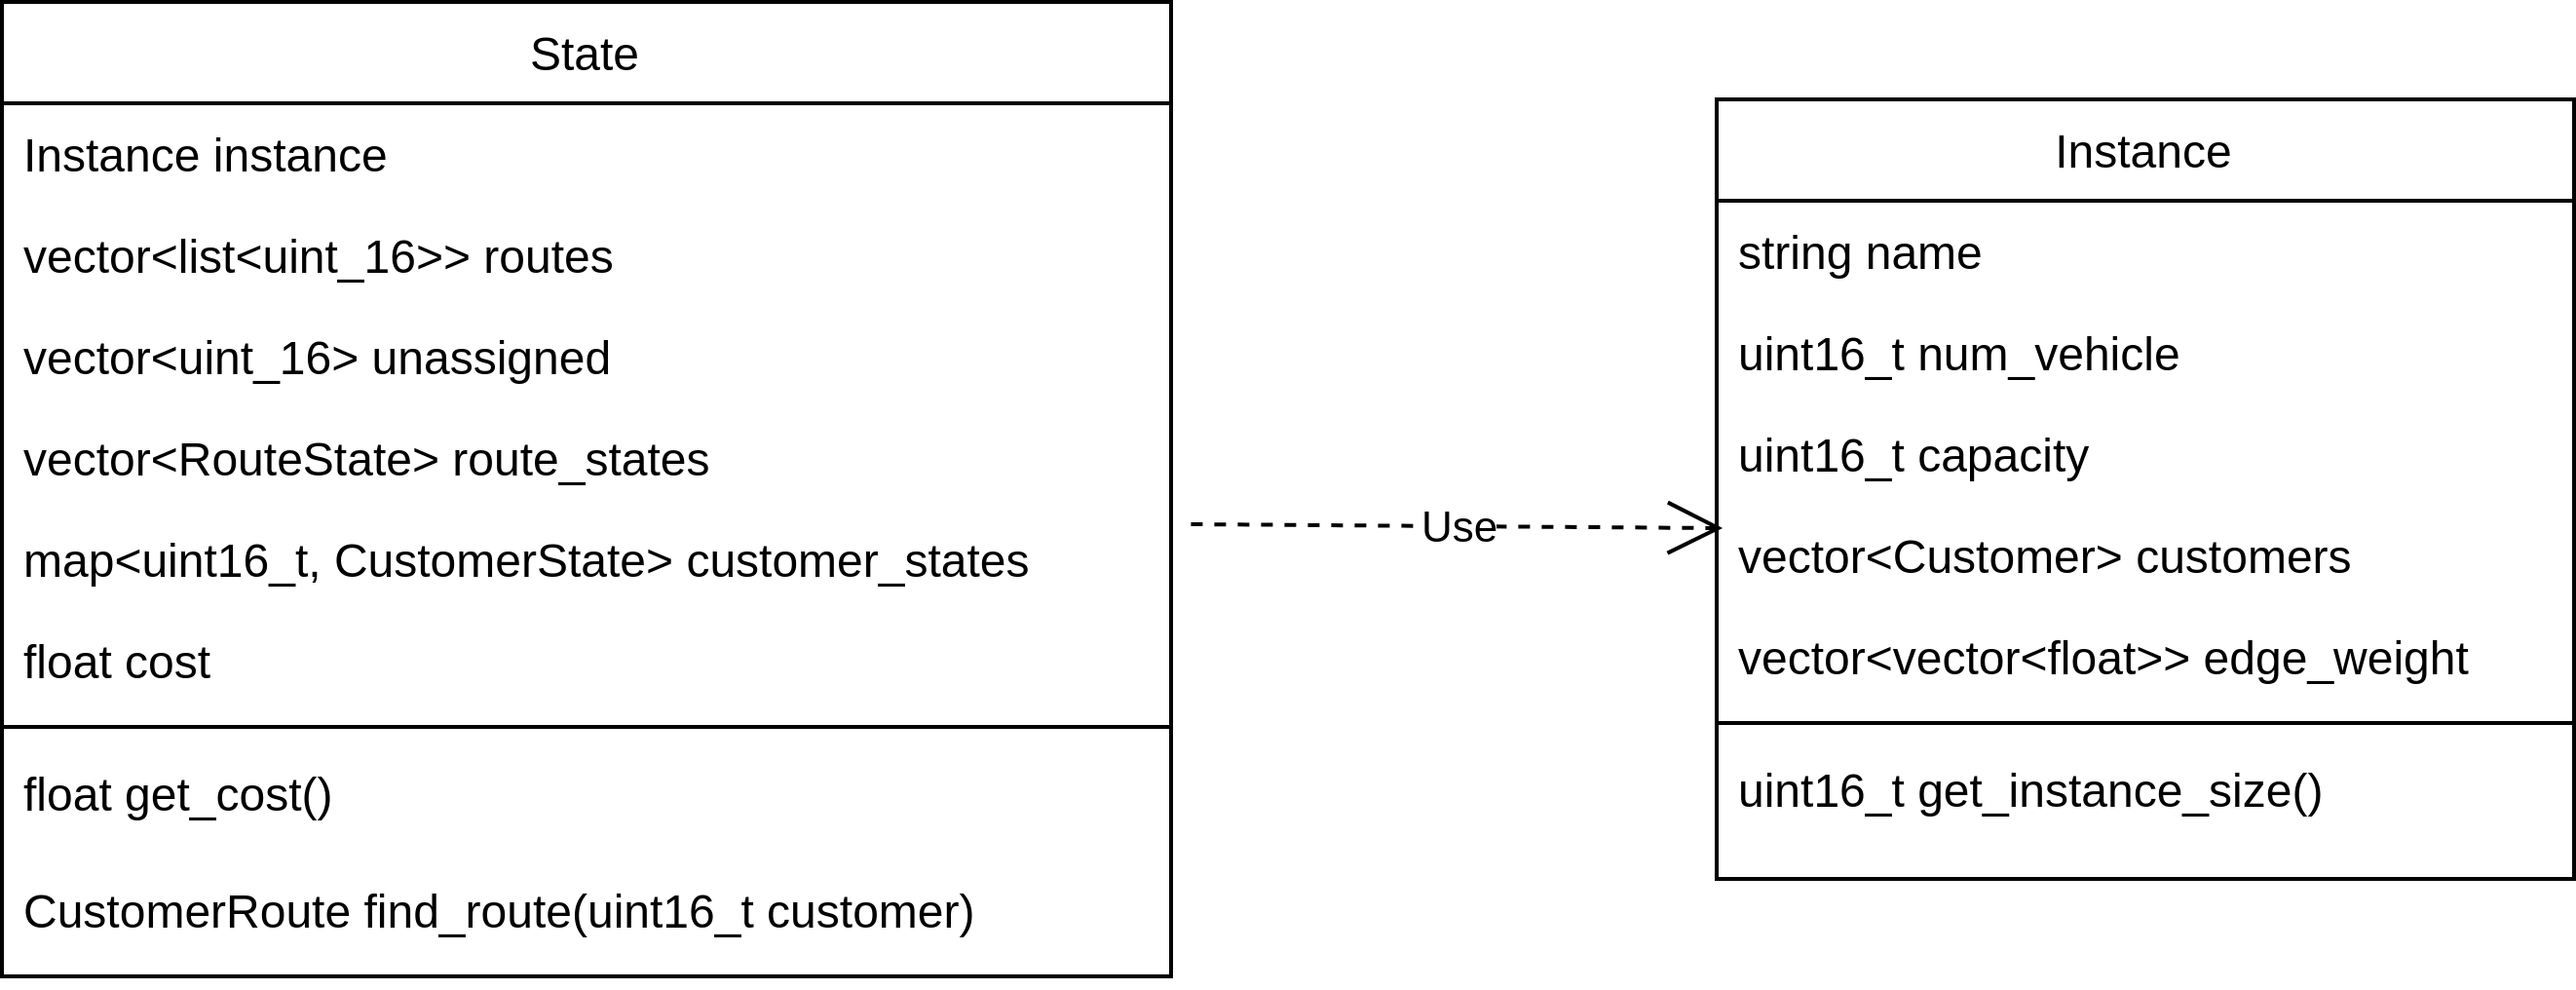
\includegraphics[width=1\textwidth]{figures/core-object.png}
    % \includesvg[scale=1]{figures/core-object}
    \caption{Lớp trạng thái của hệ}
    \label{fig:fg_04}
  \end{figure}
\end{frame}

\begin{frame}{Ứng dụng - Triển khai thuật toán}
  Chương trình được chia làm ba giai đoạn \textit{Tiền xử lý}, \textit{Chương trình chính}, \textit{Đo đạc}.
\begin{itemize}
	\item \textit{Tiền xử lý}: đọc cấu hình, tính toán ma trận khoảng cách, lưu trữ vào các tệp. 
	\item \textit{Chương trình chính}: triển khai ALNS.
	\item \textit{Đo đạc}: phân tích logs, tính toán các độ đo.
\end{itemize}
\end{frame}